% This will be the main document for the Technical Networks paper to
% be written by the Eggnet team of Jordan Ell, Triet Huynh and Braden
% Simpson in association with Adrian Schroeter and Daniela Damian.

\documentclass[conference]{IEEEtran}

% Use of outside images
\usepackage{graphicx} 

% Correct bad hyphenation here
\hyphenation{op-tical net-works semi-conduc-tor}

% Begin the paper here
\begin{document}


% Paper title
% Can use linebreaks \\ within to get better formatting as desired
\title{Finding Harmful Structures Among Developer Networks}

% Authors names
\author{\IEEEauthorblockN{Jordan Ell,
Triet Huynh,
Braden Simpson, 
Adrian Schr{\"o}ter and
Daniela Damian}
\IEEEauthorblockA{University of Victoria,
Victoria, British Columbia\\\{jell, infiro, braden\}@uvic.ca, schadr@acm.org, danielad@cs.uvic.ca}
}

% Make the title area
\maketitle


\begin{abstract}
Software systems have not only become larger over time, but the amount of
technical contributors and dependencies have also increased. With these expansions also comes
the increasing risk of introducing a software failure into a pre-existing system.
Software failures are a multi-billion dollar problem in the industry today and while integration and
other forms of testing are helping to ensure a minimal number of failures, research to understand
full impacts of changesets and their social implications is still a major concern. This paper describes
how analysis of changesets and the technical relationships they infer can be used to detect harmful
structures between contributors which may induce software failures. These harmful structures may
also be used to predict future software failures as well as provide recommendations to contributors
to solve these failures inside of changesets.
\end{abstract}


\section{Introduction}

% Setup the problem.
Large software projects are created using highly modular and 
reusable code. The problem this creates, is that methods or functions\footnote{This includes object constructors} 
can be used in a wide variety of locations throughout the project creating many technical 
dependencies.  This causes changes to any given method inside the project to have a rippling 
effect across the rest of the project~\cite{Acharya:2011:PCI}. The larger these effects are,
the more likely they are to cause a software failure inside the system during the project's
life span~\cite{Zimmermann:2008:PDU}. These observations open the door to many types
of network analysis in regard to technical dependencies and preventing software failures.

% Explain technical network research that already exists
Technical dependencies inside a project can be used to predict success or failure of 
changesets or builds~\cite{Pinzger:2008:DNP, Zimmermann:2008:PDU}. However, most 
research in this area is based off of identifying
central modules inside of a large code base which are likely to cause software failures and 
predicting future failures based on this knowledge. This method also results in predictions 
at the milestone build level of software development as opposed to a changeset level.
These research projects also lack the ability to provide recommendations.

% Introduce the idea of socio-technical congruence
Changeset failures are often also associated with the notion of a socio-technical 
congruence inside of a project~\cite{Conway:1968}. Kwan et al.~\cite{Kwan:2011:SD} shows, 
that if the build type is continuous (changesets over time), an increased level of this
congruence led to an increase in the build success probability. 

% Research question
With the power of technical dependencies in predicting software failures and the idea
that socio-technical congruence can determine changeset success, we pose the question: 
"\textit{Is it possible to locate harmful dependency structures among contributors inside
of changesets with technical dependencies and can we predict future changeset failures
while providing recommendations to solve these failures.?}"

% Explain our brief intended approach
This paper explains our attempt to create a failure prediction system on a per changeset basis using
the detection of harmful structures among developer networks.
Our process utilizes changesets and the call hierarchies effected  to find patterns of contributor 
relationships in successful and failed changesets.  We can use these contributor relationships 
to also promote the idea of socio-technical congruence with communications recommendations.


\section{Methodology}

\subsection{Extracting Technical Networks}
In order to determine whether a changeset was a success or failure (introduces a software
failure), we use the approach of Sliwerski et al.~\cite{Sliwerski:2005:CIF}.

To extract the technical dependencies of a given changeset, we first construct a method
call graph using Eclipse's ASTParser. 
Unlike  Bodden's et al.~\cite{Bodden:2003:HVJ} and other's approaches of using byte code
and whole projects, we built call graphs using source code, which does not have the assumptions
of being able to compile or have access to all project files.

We then use the Git software repository to determine what changes were made to any given
file inside of the changeset. Specifically, we look for modified methods inside of the changeset
files.

After discovering which methods have been changed, we can use the call graph to determine
which methods call those that have been changed. This creates a technical dependency between
the callers and the callee’s (changed) method. From this dependency, we can add contributors (owners) 
of the methods.

We extrapolate the owners of each method in the dependencies from the Git repository 
(Git stores contributor per line number for each file).  We now have our technical dependency 
network based on method call hierarchy with contributors (Figure~\ref{fig:network} left hand side).
We simplify the network by only using the connection between contributors since we 
are only interested in discovering the problematic edges between contributors and not the 
methods themselves (Figure~\ref{fig:network} right hand side). This is our final technical 
network.

% Technical network figure
\begin{figure*}[tb!]
\centering
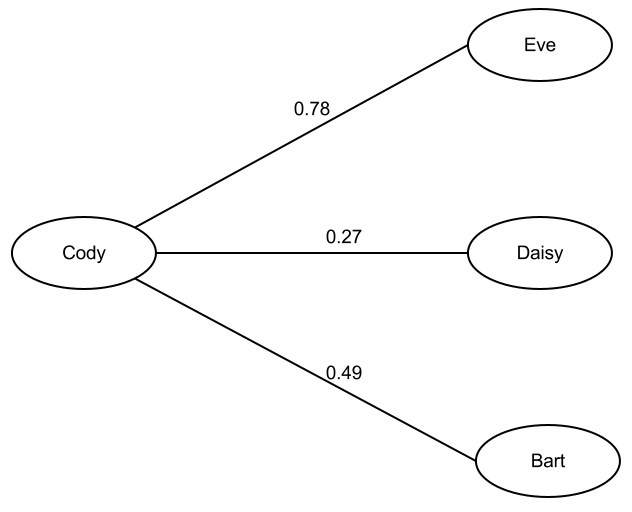
\includegraphics[width=0.9\textwidth, scale=0.5]{images/TecNetwork}
\caption{A technical network for a changeset. Cody has changed method getX() which is being
called by Bart's method foo() as well as Daisy and Adam's method bar().\label{fig:network}}
\end{figure*}

\subsection{Identifying Harmful Structures}
To identify harmful structures (edges) inside of our technical networks, we analyze these 
edges in relation to changeset failure. We proceed in the following steps:

\begin{enumerate}
\item Identify all possible edges from the technical networks.
\item For each edge, count occurrences in technical networks of failed changesets.
\item For each edge, count occurrences in technical networks of successful changesets.
\item Determine if the edge is related to success or failure.
\end{enumerate}

To determine an edge's relation to success or failure we use a Fischer Exact Value test
who's p-value is stored in our results table (Table~\ref{tab:ratio}). Pairs with the highest
p-values are said to be harmful structures inside of a project.

\section{Results}
For this paper, we choose to study the Hibernate-ORM project which is an open source Java 
application hosted on GitHub\footnote{https://github.com/}. The issue tracking for this 
project is performed by Jira\footnote{http://www.atlassian.com/software/jira/overview}.

We chose this project because it utilizes Java for all internal structures and control flow which
is ideal for creating large method call graphs. This project is also source controlled with Git
which allows the use of Git's internal tools for traversing the repository and mining
information. Finally, Hibernate-ORM uses issue tracking software which can easily be mined
using a provided API which is ideal for determining changeset success or failure.

In Hibernate-ORM, we found a total of X contributor pairs existed over the entire project, 
of which Y were found to be harmful inside of the system (A p-value of F or higher). 
We rank the pairings by their respective p-values(Table~\ref{tab:ratio}).

\begin{table}[h]
\begin{center}
\begin{tabular}{@{\hspace{.2cm}}ccc@{\hspace{.75cm}}c@{\hspace{.2cm}}}
\hline
Pair & Successful & Failed & P-Value\\
\hline
(Cody, Daisy)	&	0&	12&	1		\\
(Adam, Daisy)	&	1&	14&	0.9697	\\
(Bart, Eve)	&	2&	11&	0.9265      \\
\hline
\end{tabular}
\end{center}
\caption{The top 3 harmful contributor pairs found and ordered by failure ratio.\label{tab:ratio}}
\end{table}

By recognizing known harmful pairings in new changeset networks, we can also predict that a
given changeset will fail based on these pairings p-value. We were able to predict 
W out of Z failures from a sample size of T  given changesets inside of Hibernate-ORM 
with Q false positives. Given 
the known harmful pairing, we can also recommend communication between the two 
contributors to support the notion of socio-technical congruence.


\section{Conclusion and Future Work}
Technical dependencies are often used to predict software failures
in large software system~\cite{Pinzger:2008:DNP, Zimmermann:2008:PDU}. 
We have found evidence that technical dependencies predict failures based on contributor
dependencies found in changesets. Through the contributor dependencies,
we can also give recommendations to contributors about whom to contact to
resolve potential issues.

In future work, we will add communication networks on a per commit basis as well. We plan
to investigate the congruence of these social and technical networks and its effects on 
software quality.



\bibliographystyle{IEEEtran}
\bibliography{paper}


% End of the paper
\end{document}
